\usetheme{Madrid}
\usecolortheme{seahorse}


\graphicspath{{./images/}}

%A command for unnumbered footnotes.
%From https://latex.org/forum/viewtopic.php?t=30813
\newcommand\blfootnote[1]{%
	\begingroup
	\renewcommand\thefootnote{}\footnote{#1}%
	\addtocounter{footnote}{-1}%
	\endgroup
}

\title{An Introduction to Git}
\author{Christopher Brown}
\date{}

\begin{document}

\begin{frame}
	\titlepage
\end{frame}
\note[itemize]{
	\item
	I'm going to teach this over several sessions.
	Hopefully the first session will teach enough to just spin up a Git repository and start making commits.
	But if that's all you ever do, you're missing out on most of the benefits that version control will give you.
	So subsequent sessions will focus on how to get the most out of Git, and use it to be more productive.
}

\part{Prerequisites}

\begin{frame}
	\partpage
\end{frame}
\note[itemize]{
	\item
	Before we start looking at Git, there're some prerequisites we need to go over.
	
	\item
	Primarily, you'll need to know the very basics of the shell.
	We'll use Git from the command line (the shell), so it'll help to be familiar with it.
	
	\item
	There're also a few other things I'll explain the details of now, to save having to go off on tangents later.
}

\section{The Shell}

\subsection{Introduction}

\begin{frame}{Which Shell?}
	\begin{itemize}
		\item \texttt{sh}: the Bourne Shell by Stephen Bourne, 1977
		\item \texttt{bash}: the Bourne Again SHell, 1989
		\item \texttt{zsh}, \texttt{ksh}, \texttt{tcsh}, \texttt{rc}\dots
	\end{itemize}
	\texttt{bash} is default on most Linux distros.
	
	Mac OS X defaults to \texttt{zsh}.
	
	Git on Windows comes with a \texttt{bash} emulator.
\end{frame}
\note[itemize]{
	\item
	You might have heard of the shell called the ``terminal'' or the ``command line''.
	It's a text-based interface to your computer.
	You can use it instead of a graphical user interface (GUI).
	
	\item
	There are GUIs for Git, but it's good to know how to use it through the command line.
	
	\item
	Different shells, \texttt{bash}, \texttt{zsh}, etc.\ are mostly based on the Bourne shell.
	There are differences, but they're all similar enough that we shouldn't run into the differences here.
	
	\item
	On Linux or Mac OS X, you should be able to search for and open the ``terminal''.
	On Windows, you're looking for ``Git Bash''.
	Open it now.
}

\subsection{Navigation}

\begin{frame}{UNIX Directories}
	\begin{itemize}
		\item \texttt{/} is the root directory
		\item \texttt{cd \textasciitilde} is your user's home directory
		\begin{itemize}
			\item \texttt{/home/abc123/} on Linux
			\item \texttt{/Users/abc123/} on Mac OS X
			\item \texttt{/c/Users/abc123/} in Git Bash on Windows
		\end{itemize}
		\item \texttt{.} is the current directory
		\item \texttt{..} is the parent directory
	\end{itemize}
	Paths starting with \texttt{/} or \texttt{cd \textasciitilde} are \emph{absolute paths}.
	
	Others are \emph{relative paths}, and start from the current directory.
\end{frame}
\note[itemize]{
	\item
	The first thing to learn is how the directory structure is represented on the command line.
	Directories and files have \emph{paths}: a list, one inside the other, of the directories in the tree structure reaching down to them.
	Paths are separated by forward slashes.
	Windows sometimes uses backslashes, but Git Bash does it properly with forward slashes.
	
	\item
	The difference between absolute and relative paths is important in general.
	Generally, your code should use relative paths whenever possible.
	This is especially important in Git repositories.
	Suppose someone else downloads your repo: they'll have a different username, or put it in a different place, so the absolute path will be different.
	Use relative paths instead.
}

\begin{frame}{Moving Around}
	\begin{itemize}
		\item \texttt{pwd}: Print Working Directory
		\item \texttt{cd}: Change Directory
		\begin{itemize}
			\item \texttt{cd -} goes to previous directory
		\end{itemize}
		\item Right click in file manager to open command line there
	\end{itemize}
\end{frame}
\note[itemize]{
	\item
	At any point, your shell is in one directory: the \emph{working directory}.
	\texttt{pwd} (print working directory) will tell you which directory you're in.
	Try it now.
	
	\item
	Before we start doing anything, we'll usually want to move to the correct directory.
	We do this with \texttt{cd} (change directory).
	
	\item
	\texttt{cd} can take a relative or absolute path.
	This is when \texttt{..} to go up a directory becomes useful, and note that we can chain this or include it mid-path.
	\texttt{cd} can also take the special argument \texttt{-} to go back to the most recent working directory.
	Play around with it.
	
	\item
	You can also open the command line directly in a directory, by right-clicking in the file manager.
}

\subsection{Inspection}

\begin{frame}{Looking Around}
	\begin{itemize}
		\item \texttt{ls}: LiSt directory contents
		\begin{itemize}
			\item \texttt{ls -a} includes hidden files/directories (e.g.\ \texttt{.git}, {.gitignore})
			\item \texttt{ls -l} gives extra info
			\item \texttt{ls -al} does both
		\end{itemize}
	\end{itemize}
\end{frame}
\note[itemize]{
	\item
	When you're in a directory, you want to know which files are there.
	Or which directories, so you can \texttt{cd} further in.
	\texttt{ls} tells you.
	
	\item
	\texttt{ls} takes options, a.k.a. \emph{flags}.
	\texttt{-a} (all) shows hidden files and directories, which start with a dot.
	This is important, 'cause Git uses these.
	\texttt{-l} (long) shows owner, permissions, size, date, etc.
	
	\item
	A hyphen and a single letter is the convention for flags in the shell.
	We can combine options by giving them sequentially.
	A single hyphen followed by multiple letters also combines flags.
	Order doesn't matter.
	Demonstrate this.
	
	\item
	Some programs take long options: these use two hyphens followed by a word.
	We'll see these later on some Git commands.
}

\begin{frame}{Looking at Files}
	\begin{itemize}
		\item \texttt{cat}: print a file
		\item \texttt{head}: print the first 10 lines of a file
		\item \texttt{tail}: print the last 10 lines of a file
		\item \texttt{less}: open a file in the pager
	\end{itemize}
\end{frame}
\note[itemize]{
	\item
	There are a variety of ways we can look at the contents of a file in the command line.
	These all work within the command line, so they'll only work for text files.
	
	\item
	The names are a bit funny.
	\texttt{cat} comes from ``concatenate'', because it can print several files back-to-back.
	\texttt{less} is a better version of \texttt{more}.
}

\begin{frame}{Opening Files \& Directories}
	\begin{itemize}
		\item Open a file with the OS:
		\begin{itemize}
			\item \texttt{open} on Mac OS X
			\item \texttt{xdg-open} in Linux
			\item \texttt{start} in Git Bash on Windows
		\end{itemize}
		\item Using these on a directory opens the file manager
	\end{itemize}
\end{frame}
\note[itemize]{
	\item
	If you want to use your normal text editor, or work with non-text files, you can open files as though you'd double-clicked them in your file manager.
	How to do this differs by OS.
	
	\item
	You can also use these to open your file manager, which can be helpful to move or copy files if you're not familiar with doing so on the command line.
}

\subsection{Modification}

\begin{frame}{Changing Things}
	\begin{itemize}
		\item \texttt{mkdir}: MaKe DIRectory
		\item \texttt{rmdir}: ReMove empty DIRectory
		\item \texttt{touch}: create blank file, or change last modified date
		\item \texttt{cp}: CoPy a file
		\begin{itemize}
			\item \texttt{cp -r}: CoPy a directory (recursive)
		\end{itemize}
		\item \texttt{mv}: MoVe/rename a file/directory
		\item \texttt{rm}: ReMove a file
		\begin{itemize}
			\item \texttt{rm -i} asks confirmation: safer
			\item \texttt{rm -r} removes a directory and everything inside: DANGER!
		\end{itemize}
	\end{itemize}
\end{frame}
\note[itemize]{
	\item
	We can use all sorts of commands to create, remove, copy, or remove files or directories.
	I won't go into the details now, and you should be able to do most of this with your file manager.
	But this might be useful in future, and you might see me using these out of habit.
}

\section{Hashes}

\subsection{SHA1}

\begin{frame}{Hashing}
	\centering
	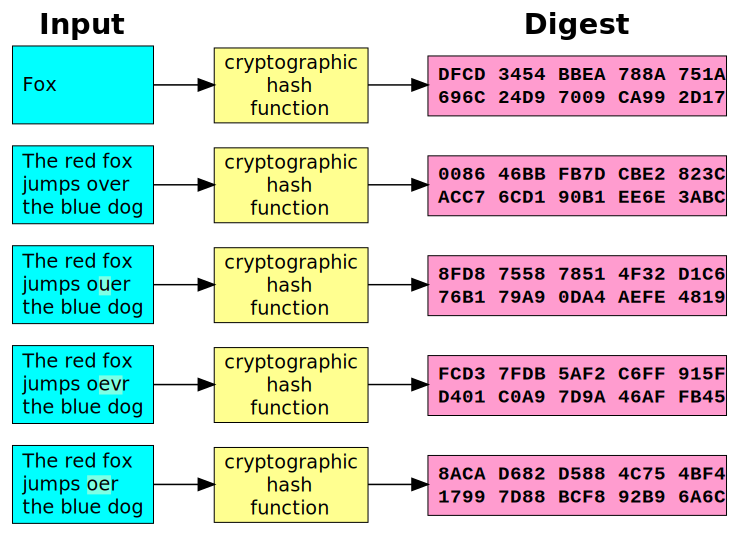
\includegraphics[width=\textwidth,height=0.8\textheight,keepaspectratio]{sha1}
	\blfootnote{Cryptographic Hash Function by Jorge Stolfi}
\end{frame}
\note[itemize]{
	\item
	A hash function converts some arbitrary input to a fixed-length string of seemingly-random input.
	It always converts the same input to the same output.
	But small changes in input cause large changes in output.
	
	\item
	This example uses the SHA1 hash function, the same one used by Git.
	We'll get to why Git needs this later.
	
	\item
	You can use \texttt{sha1sum} at your command line.
	(Demonstrate this a bit.)
	
	\item
	Note that you can use this hash huge files, and still get a fixed-length output.
	It's theoretically possible for two different files to give the same output, but astronomically unlikely.
}

\subsection{Uses}

\begin{frame}{Uses of Hashes}
	\begin{itemize}
		\item Checksums: checking download validity
		\item Security: storing passwords
		\item Version control: identifying versions
	\end{itemize}
\end{frame}
\note[itemize]{
	\item
	Hashes have a bunch of different uses.
	
	\item
	Suppose you download a huge file, and you want to know if the download got corrupted.
	The server hashes the file, and you hash the file, and you compare hashes.
	If one small bit in the file is wrong, the hash will be totally different.
	
	\item
	Websites that need a password should never store your password in plain text.
	If they did, and they got hacked, your password would be available for everyone to see.
	Instead, they store a hash of your password.
	When you submit your password, they check the hash of that against their stored hash.
	Hashes are not easily reversible, so someone who hacks the server and gets the hash can't easily get your original password.
	
	\item
	Our use is in version control.
	You can hash a file.
	Then, to check if the file's changed, you can just hash it again and check if the hash has changed.
}

\part{Introduction to Git}

\begin{frame}
	\partpage
\end{frame}
\note[itemize]{
	\item
	With that out of the way, it's time to start explaining Git itself.
	That said, I'll be beginning with quite a lot of motivation and background before we get into the actual commands, so bear with me.
}

\section{Motivation}

\subsection{General Use}

\begin{frame}{Why Use Git?}
	\centering
	\includegraphics[width=\textwidth,height=0.8\textheight,keepaspectratio]{phd-final}
	\blfootnote{Piled Higher and Deeper by Jorge Cham}
\end{frame}
\note[itemize]{
	\item
	Why do we use Git?
	The main things is that it allows us to keep different versions in a well-controlled fashion.
	It avoids the stereotypical proliferation of poorly named ``final'' versions.
	
	\item
	It's also very useful for any sort of collaborative effort.
	Have you ever done any sort of collaborative project where you're emailing files back and forth.
	Nobody can keep track of which is the most recent version.
	And if you both change a file at the same time, how do you combine the versions?
	Git handles the versioning for you, and also has a very neat algorithm for merging two sets of changes into a version with both changes.
	
	\item
	Version control is also very useful for reproducible research.
	When you share a paper, you can use version control to provide a snapshot of the code that produced it.
	Then, even if you keep working on that code, that snapshot exists for you or others to reproduce that work.
}

\subsection{Fixing Problems}

\begin{frame}{What Can Git Do?}
	\begin{itemize}
		\item What have other people changed since I last worked on this?
		\begin{itemize}
			\item \texttt{git log}
		\end{itemize}
		\item I changed some stuff, and my supervisor changed some other stuff, and I need to combine them
		\begin{itemize}
			\item \texttt{git merge}
		\end{itemize}
		\item I want to try something, but I'm worried it'll break stuff
		\begin{itemize}
			\item \texttt{git branch}
		\end{itemize}
		\item Everything I've just done has made things worse; I want to go back to how it was
		\begin{itemize}
			\item \texttt{git reset --hard} (or \texttt{git stash})
		\end{itemize}
		\item This was working fine a week ago, but now it's broken
		\begin{itemize}
			\item \texttt{git bisect}
		\end{itemize}
		\item What was I thinking when I wrote this line?
		\begin{itemize}
			\item \texttt{git blame}
		\end{itemize}
	\end{itemize}
\end{frame}
\note[itemize]{
	\item
	Git can do a lot more than just the standard storing and sharing of versions.
	It has a lot of benefits even just for a solo developer.
	Today, I'm going to focus mostly on just getting you working with Git.
	But next session, we'll go over some of the really helpful things you can do with it.
	
	\item
	In the meantime, here's a taste of some of the things we can do with Git.
	Have you ever found yourself in any of these situations?
	Git has commands to solve them.
}

\section{The Git Parable}

\subsection{The Parable}

\begin{frame}{How Not To Explain Git}
	\centering
	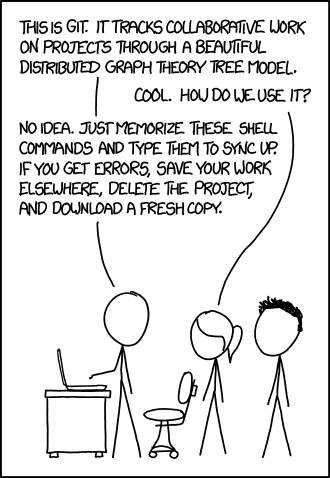
\includegraphics[width=\textwidth,height=0.8\textheight,keepaspectratio]{xkcd-git}
	\blfootnote{xkcd by Randall Munroe}
\end{frame}
\note[itemize]{
	\item
	A lot of people teach Git by this method: they show the standard \texttt{pull}, \texttt{add}, \texttt{commit}, \texttt{push} workflow, and leave it at that.
	The problem with doing this is that, while it allows you to work with other people who use Git, you get very little benefit from using Git that way.
	You won't understand enough to do any of the cool and useful things I just demonstrated.
}

\begin{frame}{How To Explain Git}
	The Git Parable, by Tom Preston-Werner
	\begin{itemize}
		\item \url{https://tom.preston-werner.com/2009/05/19/the-git-parable.html}
	\end{itemize}
	Suppose you only have a text editor and a file manager.
	How would you develop version control?
\end{frame}
\note[itemize]{
	\item
	Instead, I'm going to explain how Git actually works.
	It can appear quite complicated, so we're going to build it from the ground up.
	I'm shamelessly stealing from the best explanation of Git I've seen: ``the Git Parable'', by Tom Preston--Werner, co-founder of GitHub.
	
	\item
	The Git Parable works as follows.
	Suppose Git doesn't exist; suppose you don't have any fancy software at all.
	You've just got a text editor and a file manager, and you're setting out on a massive coding project that you need to version control.
	How, with just your text editor and file manager, would you control your versions?
}

\end{document}
